\section{Methodology}
\label{sec:methodology}
\begin{figure*}[!t]
\centering
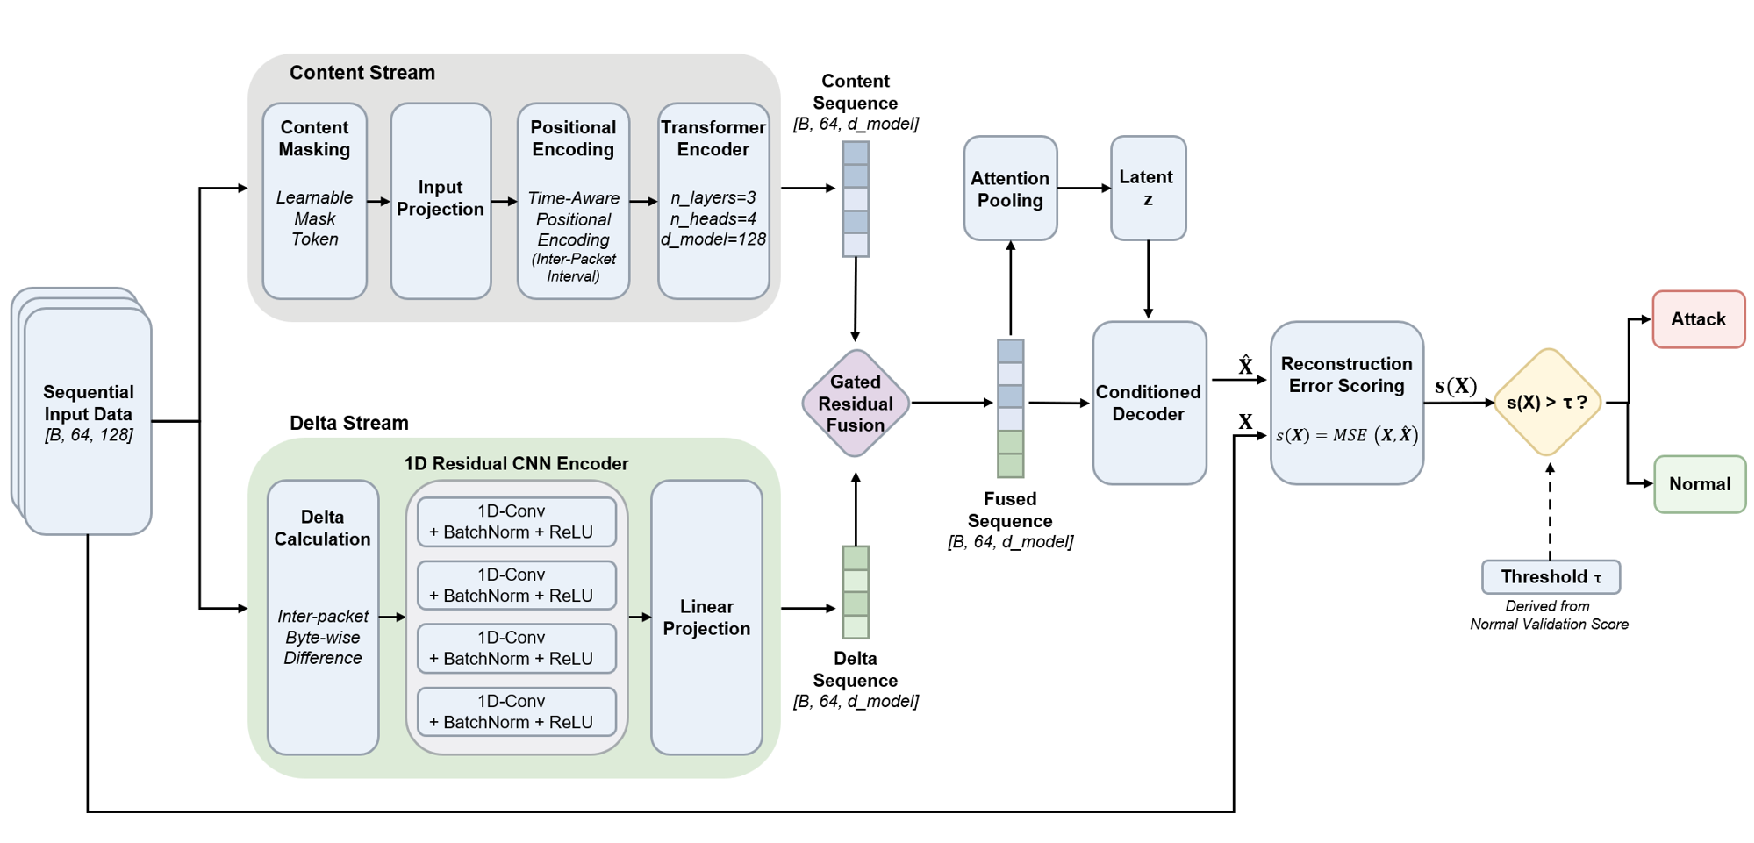
\includegraphics[width=\textwidth]{figs/architecture.pdf}
\caption{Overview of the proposed dual-stream masked autoencoder. The content stream (Transformer) is conditioned on both the masked packet content and a time-aware positional encoding derived from inter-packet capture timestamps; the delta stream (residual 1D-CNN) processes inter-packet byte differences. The two streams are combined through delta-conditioned gated residual fusion, after which attention pooling produces a global latent vector $\mathbf{z}$ that, together with the fused sequence representation $\mathbf{F}$, conditions the decoder's reconstruction. At inference, the mean reconstruction error $s(\mathbf{X})$ is compared against a validation-derived threshold $\tau$ to flag intrusions. Equation numbers refer to their first appearance in Section~\ref{sec:methodology}.}
\label{fig:architecture}
\end{figure*}

\subsection{Problem Formulation}
\begin{figure}[]
\centering
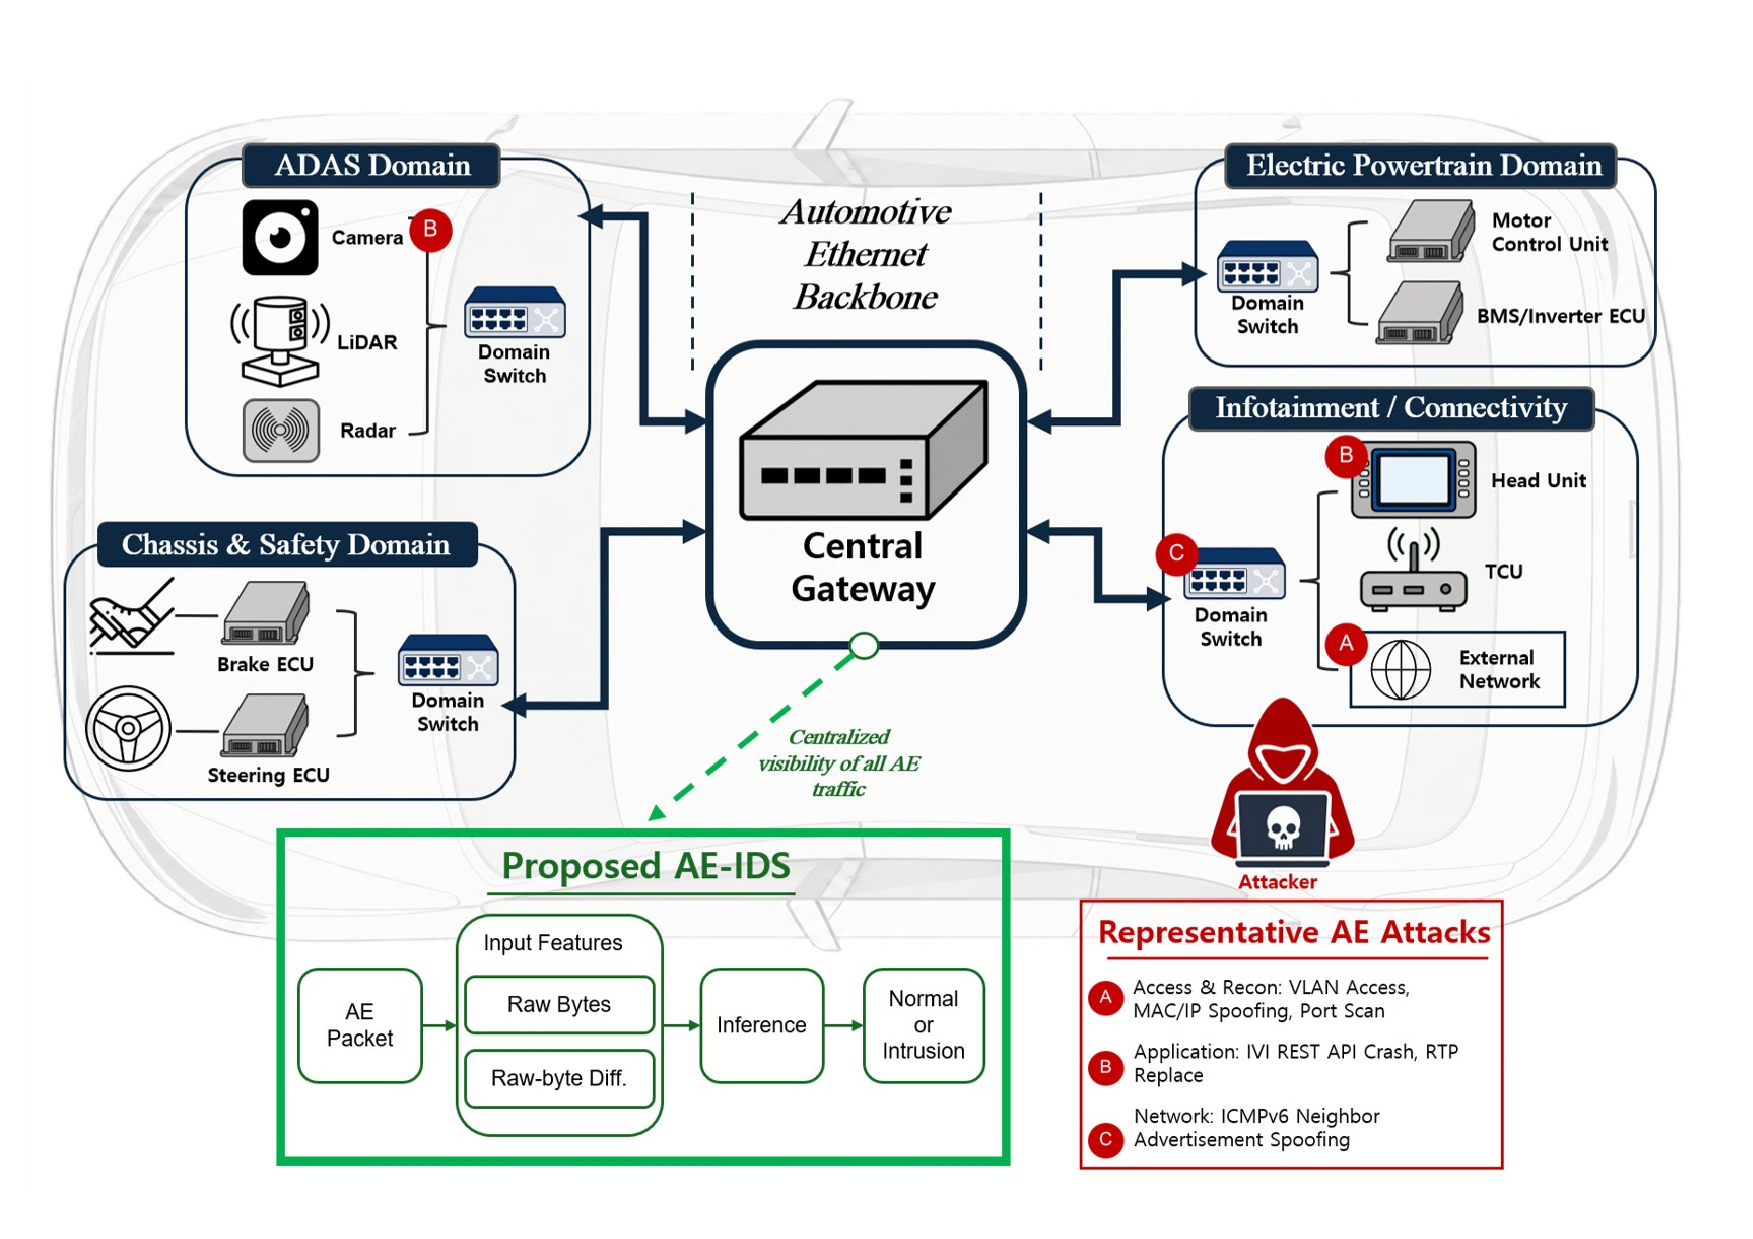
\includegraphics[width=\columnwidth]{figs/proposed_ids_architecture.pdf}
\caption{\textcolor{red}{Conceptual deployment of the proposed AE-IDS in a domain-based in-vehicle network. The ADAS, chassis and safety, electric powertrain, and infotainment/connectivity domains exchange inter-domain traffic through the Automotive Ethernet backbone and central gateway. The proposed detector passively analyzes gateway-visible AE packets using raw bytes and inter-packet raw-byte differences. The labeled markers summarize the representative CarDS attack scenarios considered in this work: (A) network access and reconnaissance, (B) application-layer exploitation, and (C) network-layer neighbor spoofing.}}
\label{fig:ae_deployment}
\end{figure}

\textcolor{red}{Figure~\ref{fig:ae_deployment} illustrates the intended deployment context of the proposed method. The four domains provide a conceptual functional partition of a modern electric vehicle rather than an exact reconstruction of a particular production topology. The ADAS domain contains high-bandwidth sensors, the chassis and safety domain contains safety-critical control ECUs, the electric powertrain domain contains the motor-control and battery/inverter ECUs, and the infotainment/connectivity domain contains the head unit, telematics control unit, and external-network interfaces. Their inter-domain AE traffic is forwarded through the central gateway, making the gateway a suitable centralized observation point for vehicle-wide intrusion detection.}

\textcolor{red}{The AE-IDS is assumed to receive a passive copy of the AE packets observable at the central gateway, for example through an internal monitoring interface, switch-port mirroring, or a passive tap. It therefore does not participate in packet forwarding and does not introduce additional control-path latency. The phrase \emph{centralized visibility} refers specifically to traffic that traverses, or is mirrored to, the gateway; traffic exchanged only within a local switched domain is observable only if the corresponding domain switch exports a copy to this monitoring point. This deployment assumption makes the monitoring coverage explicit while preserving the protocol-agnostic packet representation used by the detector.}

\textcolor{red}{The A--C markers in Figure~\ref{fig:ae_deployment} indicate where representative Automotive Ethernet attacks can enter or affect the network. Marker A denotes access and reconnaissance activity originating from the externally connected infotainment/connectivity domain, including unauthorized VLAN access, MAC/IP spoofing, and TCP port scanning. Marker B denotes the CarDS application-layer attacks: exploitation of an IVI REST API at the head unit and replacement of an unprotected RTP camera stream. The camera marker therefore represents the attacked video stream and does not imply that the same RTP-specific attack is directly applicable to LiDAR or radar traffic; attacks against those sensors would require protocol-specific injection or replay mechanisms. Marker C denotes forged ICMPv6 Neighbor Advertisement messages that manipulate the internal switch's neighbor/forwarding state and redirect traffic toward the attacker. Collectively, these attacks alter Ethernet headers, addressing and protocol fields, transport behavior, or application payloads. This motivates processing both the raw packet bytes and their consecutive byte-wise differences: the former preserves the complete packet content, while the latter emphasizes abrupt local changes introduced by spoofing, scanning, and frame replacement.}

We formulate Automotive Ethernet intrusion detection as an unsupervised anomaly detection problem. Let a raw packet be represented as a byte sequence $\mathbf{p}_i \in \{0, \ldots, 255\}^{L}$, where $L = 128$ denotes the maximum byte length, with zero-padding applied to packets shorter than $L$. Each byte value is normalized to $[0, 1]$ by dividing by 255. A traffic window is defined as a temporally ordered sequence of $N = 64$ consecutive packets, $\mathbf{X} = [\mathbf{p}_1, \mathbf{p}_2, \ldots, \mathbf{p}_N] \in \mathbb{R}^{N \times L}$, constructed using a sliding window of stride 1 over the full packet stream.

A window-level binary label $y \in \{0, 1\}$ is assigned during evaluation only: $y = 1$ if at least one packet within the window is malicious, and $y = 0$ otherwise. The model is trained exclusively on windows drawn from normal traffic ($y = 0$) and receives no label information during training. The objective is to learn a function $f: \mathbb{R}^{N \times L} \rightarrow \mathbb{R}_{\geq 0}$ that assigns a scalar anomaly score to each window such that anomalous windows receive systematically higher scores than normal windows. At inference time, a window is classified as an intrusion if its anomaly score exceeds a threshold $\tau$ derived from the normal traffic distribution.

\noindent\textit{Notational convention.} Throughout this section, all vector and matrix quantities follow the row-vector convention, in which a linear projection is written as $\mathbf{Y} = \mathbf{X}\mathbf{W} + \mathbf{b}$ with $\mathbf{W} \in \mathbb{R}^{d_{\text{in}} \times d_{\text{out}}}$. Sequence-level quantities (e.g., $\mathbf{X}, \mathbf{C}, \mathbf{D}, \mathbf{F}$) are treated as $N \times d$ matrices whose rows correspond to individual packets, while window-level quantities that collapse the sequence into a single vector (e.g., $\bar{\mathbf{z}}, \mathbf{z}$) are treated as $1 \times d$ row vectors under the same convention.



\subsection{Overview of the Proposed Method}
The proposed method consists of three components: (1) a dual-stream encoder that produces a latent representation of the input window, (2) a masked reconstruction objective used for self-supervised training, and (3) a threshold-based anomaly scoring mechanism used at inference time. An overview of the full architecture is shown in Figure~\ref{fig:architecture}.

The dual-stream encoder processes the input window $\mathbf{X}$ through two parallel streams. The \textbf{content stream} applies a Transformer encoder to the raw byte content of each packet, modeling global inter-packet dependencies across the full window; rather than the conventional fixed sinusoidal positional encoding, the content stream is conditioned on the actual inter-packet timing recorded at capture time, allowing it to reason jointly about packet content and packet timing. The \textbf{delta stream} applies a residual 1D-CNN encoder to the inter-packet byte difference sequence, modeling per-byte temporal dynamics across consecutive packets. The content stream serves as the primary carrier of discriminative information, while the delta stream acts as a self-gated auxiliary signal that supplements it with local temporal cues. The outputs of both streams are fused through a delta-conditioned gated residual mechanism and aggregated via attention pooling to produce a compact latent vector $\mathbf{z}$. A conditioned sequence decoder then reconstructs the original packet content from the fused sequence representation and $\mathbf{z}$. Table~\ref{tab:notation} summarizes the notation used throughout this section.

\begin{table}[!t]
\centering
\caption{Summary of notation.}
\label{tab:notation}
\footnotesize
\begin{tabular}{cp{0.7\columnwidth}}
\toprule
\textbf{Symbol} & \textbf{Description} \\
\midrule
$N, L$                          & window size (64), byte length (128) \\
$\mathbf{p}_i$                  & raw content of packet $i$ \\
$\mathbf{\Delta X}_i$           & inter-packet byte difference at $i$ \\
$\iota_i$                       & inter-packet interval (IPI) at $i$ \\
$\mathbf{m}, m_i$                & packet-level mask vector / indicator \\
$\mathbf{e}_{\text{mask}}$      & learnable mask token \\
$\mathbf{P}, \mathbf{T}$        & sinusoidal, time-aware positional encoding \\
$\mathbf{C}, \mathbf{D}$        & content-, delta-stream outputs \\
$\mathbf{F}$                    & fused sequence representation \\
$\bar{\mathbf{z}}, \mathbf{z}$  & pooled, refined latent vector \\
$\hat{\mathbf{p}}_i$            & reconstructed content of packet $i$ \\
$\tau$                          & anomaly detection threshold \\
\bottomrule
\end{tabular}
\end{table}

\subsection{Input Representation}

\noindent\textbf{Raw Content Input.}
The content stream receives the normalized window $\mathbf{X} \in \mathbb{R}^{N \times L}$ directly as input, where each row $\mathbf{p}_i \in \mathbb{R}^{L}$ represents the normalized byte content of the $i$-th packet.

\noindent\textbf{Delta Input.}
The delta stream receives the inter-packet byte difference sequence $\mathbf{\Delta X} \in \mathbb{R}^{N \times L}$, computed as
\begin{equation}
    \mathbf{\Delta X}_i =
    \begin{cases}
        \mathbf{0} & \text{if } i = 1 \\
        \mathbf{p}_i - \mathbf{p}_{i-1} & \text{if } i > 1.
    \end{cases}
    \label{eq:delta}
\end{equation}
The delta sequence captures how each byte position evolves across consecutive packets. Under normal traffic, protocol fields such as sequence numbers exhibit predictable incremental patterns; anomalous traffic introduces irregular byte-level fluctuations at specific positions that are more salient in the delta domain than in the raw content domain.

\noindent\textbf{Temporal Input.}
In addition to byte-level content and delta, we incorporate inter-packet timing as a third input modality. Let $t_i$ denote the capture timestamp of packet $i$. The inter-packet interval (IPI) sequence $\boldsymbol{\iota} \in \mathbb{R}^{N \times 1}$ is computed as
\begin{equation}
    \iota_i =
    \begin{cases}
        0 & \text{if } i = 1 \\
        \log\!\left(1 + |t_i - t_{i-1}|\right) & \text{if } i > 1,
    \end{cases}
    \label{eq:ipi}
\end{equation}

mirroring the zero-initialization convention used for the delta sequence [Eq.~\eqref{eq:delta}]. The logarithmic compression $\log(1+|\cdot|)$ accounts for the wide dynamic range of Automotive Ethernet inter-arrival times, which span several orders of magnitude (microseconds to seconds) depending on traffic type and driving scenario; without this compression, occasional large inter-arrival gaps would dominate the learned representation. The IPI sequence is derived solely from packet capture timestamps and is independent of any upper-layer protocol parsing, preserving the protocol-agnostic nature of the proposed method.

\noindent\textbf{Masking.}
Prior to encoding, a packet-level binary mask $\mathbf{m} \in \{0, 1\}^{N}$ is sampled to determine which packets within the window are masked: each position $i \in \{1, \ldots, N\}$ is independently drawn as $m_i \sim \text{Bernoulli}(p_{\text{mask}})$ with $p_{\text{mask}} = 0.20$, so that approximately 20\% of the $N$ packets in each window are selected for masking. For each position where $m_i = 1$, the entire $L$-dimensional content vector $\mathbf{p}_i$ is replaced --- not with random values, but with a single shared, learned mask token $\mathbf{e}_{\text{mask}} \in \mathbb{R}^{L}$, initialized from $\mathcal{N}(0, 0.02^2)$ and updated during training via backpropagation:
\begin{equation}
    \tilde{\mathbf{p}}_i =
    \begin{cases}
        \mathbf{e}_{\text{mask}} & \text{if } m_i = 1 \\
        \mathbf{p}_i             & \text{if } m_i = 0.
    \end{cases}
    \label{eq:mask}
\end{equation}

This design follows the masked autoencoding paradigm of BERT~\cite{devlin2019bert} and MAE~\cite{he2022masked}, where the \emph{location} of masking is randomized while the \emph{substituted value} is a single learnable embedding shared across all masked positions, rather than random noise. The delta input is computed from the original unmasked content [Eq.~\eqref{eq:delta}] and is not subject to masking, preserving the integrity of the variation signal. Similarly, the IPI sequence $\boldsymbol{\iota}$ [Eq.~\eqref{eq:ipi}] is left unmasked at every position, including $i$ with $m_i = 1$: only the byte-level content vector $\mathbf{p}_i$ is replaced by $\mathbf{e}_{\text{mask}}$, while the timing signal used to compute $\mathbf{P}_{\text{enc}}$ remains the true inter-packet interval. This mirrors standard practice in masked autoencoding architectures, where positional encodings are treated as always-visible structural context rather than maskable content; masking the timing signal itself would additionally confound the reconstruction objective, since the decoder would then have to infer both the missing content and the missing timing of a packet from a single shared mask token.

\subsection{Dual-Stream Encoder}
\subsubsection{Content Stream: Transformer Encoder}
The content stream models global inter-packet dependencies using a standard Transformer encoder~\cite{vaswani2017attention}. Let $\tilde{\mathbf{X}} = [\tilde{\mathbf{p}}_1, \ldots, \tilde{\mathbf{p}}_N]$ denote the masked window from Eq.~\eqref{eq:mask}. The masked content input is first projected to the model dimension $d_{\text{model}} = 128$ via a linear layer, after which a positional encoding matrix $\mathbf{P}_{\text{enc}} \in \mathbb{R}^{N \times d_{\text{model}}}$ is added to inject positional information:
\begin{equation}
    \mathbf{H}^{(0)}_c = \text{Dropout}\!\left( \tilde{\mathbf{X}}\mathbf{W}_c + \mathbf{b}_c + \mathbf{P}_{\text{enc}} \right) \in \mathbb{R}^{N \times d_{\text{model}}},
    \label{eq:posenc}
\end{equation}

where $\mathbf{W}_c \in \mathbb{R}^{L \times d_{\text{model}}}$ is the projection weight and $\text{Dropout}(\cdot)$ is applied at rate $p_{\text{drop}} = 0.1$. The same rate $p_{\text{drop}} = 0.1$ is used uniformly across the network: in Eq.~\eqref{eq:posenc} above, inside each Transformer encoder layer of Eq.~\eqref{eq:transformer}, and in the latent refinement step of Eq.~\eqref{eq:latent}. We consider two schemes for instantiating $\mathbf{P}_{\text{enc}}$, compared directly in the ablation study of Section~\ref{sec:ablation}.

\noindent\textit{Sinusoidal positional encoding (baseline).} Following the conventional Transformer scheme~\cite{vaswani2017attention}, $\mathbf{P}_{\text{enc}} = \mathbf{P}$ is a fixed matrix computed from each packet's discrete rank $i \in \{1, \ldots, N\}$ within the window using the standard sine/cosine basis. This scheme encodes only the \emph{ordinal position} of a packet (0th, 1st, \ldots, 63rd) and is invariant to the actual elapsed time between packets.

\noindent\textit{Time-aware positional encoding (proposed).} Automotive Ethernet attacks such as high-rate port scanning, packet replay, and flooding typically manifest as anomalous \emph{inter-arrival timing} rather than anomalous sequence rank, a signal that the sinusoidal scheme cannot represent. We therefore propose conditioning the positional signal directly on the IPI sequence $\boldsymbol{\iota}$ [Eq.~\eqref{eq:ipi}] via a learnable projection:
\begin{equation}
    \mathbf{P}_{\text{enc}} = \mathbf{T} =
    \text{GELU}\!\left(\boldsymbol{\iota}\mathbf{W}_{t_1} + \mathbf{b}_{t_1}\right)\mathbf{W}_{t_2} + \mathbf{b}_{t_2},
    \label{eq:timepe}
\end{equation}

with $\mathbf{T} \in \mathbb{R}^{N \times d_{\text{model}}}$, $\mathbf{W}_{t_1} \in \mathbb{R}^{1 \times d_{\text{model}}}$ and $\mathbf{W}_{t_2} \in \mathbb{R}^{d_{\text{model}} \times d_{\text{model}}}$. Unlike the fixed sinusoidal matrix $\mathbf{P}$, the time-aware encoding $\mathbf{T}$ is differentiable and learns to map raw timing irregularities directly into the representation space, replacing ``\emph{which position is this packet}'' with ``\emph{how much time elapsed before this packet arrived}'' as the positional signal injected into the content stream. Unless otherwise noted, the time-aware scheme is adopted as the default configuration for the results reported in this paper; the sinusoidal scheme is retained as an ablation baseline to isolate its contribution.

The projected sequence $\mathbf{H}^{(0)}_c$ is passed through $n_{\text{layers}} = 3$ Transformer encoder layers with pre-layer normalization, each consisting of multi-head self-attention with $n_{\text{head}} = 4$ heads and a position-wise feed-forward network with hidden dimension $d_{\text{ff}} = 256$:
\begin{equation}
    \mathbf{C} = \text{TransformerEncoder}(\mathbf{H}^{(0)}_c) \in \mathbb{R}^{N \times d_{\text{model}}}.
    \label{eq:transformer}
\end{equation}

The Transformer encoder is suited to the content stream because inter-packet dependencies in Automotive Ethernet traffic are inherently global: the anomalous nature of a given packet may be most apparent in relation to temporally distant packets, such as when a scanning sequence targets non-consecutive port ranges across the window. This global receptive field also motivates injecting timing information specifically into the content stream rather than the delta stream: because self-attention computes interactions among all $N$ packets jointly, an anomalously short or long inter-packet interval can be weighed by attention relative to the timing of every other packet in the window. In contrast, the delta stream's convolutional kernels (size 3--5) only relate a packet to its immediate neighbors, limiting their ability to contextualize timing irregularities against the full window.

\subsubsection{Delta Stream: Residual CNN Encoder}
The delta stream captures local temporal change patterns at each byte position using a residual one-dimensional convolutional neural network. Since each byte position across $N$ consecutive packets constitutes an independent temporal signal, the delta sequence $\mathbf{\Delta X} \in \mathbb{R}^{N \times L}$ from Eq.~\eqref{eq:delta} is transposed to $\mathbb{R}^{L \times N}$, treating each byte position as a channel and the packet index as the sequence axis. The transposed input is processed by a stack of residual convolutional blocks with filter progression $[128, 128, 128, C_{\text{last}}]$, $C_{\text{last}} = 64$:
\begin{equation}
    \mathbf{D}' = \text{ResidualCNN}\!\left(\mathbf{\Delta X}^{\top}\right) \in \mathbb{R}^{C_{\text{last}} \times N}.
    \label{eq:cnn}
\end{equation}

Each residual block applies two successive 1D convolutions with kernel size 3 (kernel size 5 in the final block), batch normalization, and ReLU activation, with a $1\times1$ convolutional skip connection applied whenever the input and output channel dimensions differ. Formally, letting $\mathbf{U}^{(l-1)}$ denote the input to the $l$-th block ($\mathbf{U}^{(0)} = \mathbf{\Delta X}^{\top}$), each block computes
{\footnotesize
\begin{multline}
    \mathbf{U}^{(l)} = \text{ReLU}\!\Big(\text{BN}\big(\text{Conv}_2^{(l)}(\text{ReLU}(\text{BN}(\text{Conv}_1^{(l)}(\mathbf{U}^{(l-1)}))))\big) \\
    {}+ \mathbf{S}^{(l)}\big(\mathbf{U}^{(l-1)}\big)\Big),
    \label{eq:resblock}
\end{multline}
}
where $\text{Conv}_1^{(l)}, \text{Conv}_2^{(l)}$ are the block's two 1D convolutions, $\text{BN}(\cdot)$ denotes batch normalization, and $\mathbf{S}^{(l)}(\cdot)$ is the skip path: the identity map if the input and output channel dimensions of block $l$ match, and a $1\times1$ convolution followed by batch normalization otherwise. Stacking $n_{\text{blocks}} = 4$ such blocks with channel progression $[128, 128, 128, C_{\text{last}}]$ ($C_{\text{last}} = 64$) yields $\mathbf{D}' = \mathbf{U}^{(n_{\text{blocks}})}$, consistent with the $\text{ResidualCNN}(\cdot)$ notation of Eq.~\eqref{eq:cnn} above. The output is then transposed back to sequence-first format and linearly projected to $d_{\text{model}}$:
\begin{equation}
    \mathbf{D} = {\mathbf{D}'}^{\top}\mathbf{W}_d + \mathbf{b}_d \in \mathbb{R}^{N \times d_{\text{model}}},
    \label{eq:deltaproj}
\end{equation}

where $\mathbf{W}_d \in \mathbb{R}^{C_{\text{last}} \times d_{\text{model}}}$ and $\mathbf{b}_d \in \mathbb{R}^{d_{\text{model}}}$.
This design allows the CNN to independently track how each byte position evolves over the packet sequence. By applying convolutional kernels along the packet axis with a local receptive field, the model efficiently detects position-specific anomalies --- such as irregular fluctuations in byte offsets corresponding to source addresses, port numbers, or RTP sequence fields --- that manifest as abrupt local deviations in the delta domain.

\begin{algorithm}[!t]
\caption{Self-Supervised Dual-Stream Masked Reconstruction Training}
\label{alg:training}
\begin{algorithmic}[1]
\REQUIRE Normal traffic windows $\{\mathbf{X}^{(k)}\}_{k=1}^{K_{\text{train}}}$, mask probability $p_{\text{mask}}$, masked-loss weight $\lambda$, max epochs $E$, patience $P$
\ENSURE Trained encoder-decoder parameters $\theta^\star$
\STATE Initialize model parameters $\theta$, including mask token $\mathbf{e}_{\text{mask}} \sim \mathcal{N}(0, 0.02^2)$
\STATE $b_{\text{best}} \gets \infty$; $c \gets 0$
\FOR{epoch $= 1$ \TO $E$}
    \FOR{each mini-batch $\{\mathbf{X}^{(k)}\}$ from training set}
        \STATE Compute delta sequence $\mathbf{\Delta X}^{(k)}$ via Eq.~\eqref{eq:delta} and IPI sequence $\boldsymbol{\iota}^{(k)}$ via Eq.~\eqref{eq:ipi}
        \STATE Sample packet-level mask $\mathbf{m}^{(k)} \sim \text{Bernoulli}(p_{\text{mask}})$ and apply Eq.~\eqref{eq:mask}
        \STATE Encode content stream $\mathbf{C}$ [Eqs.~\eqref{eq:posenc}--\eqref{eq:transformer}, with $\mathbf{P}_{\text{enc}} = \mathbf{T}$ from Eq.~\eqref{eq:timepe}] and delta stream $\mathbf{D}$ [Eq.~\eqref{eq:deltaproj}]
        \STATE Fuse streams into $\mathbf{F}$ via gated residual fusion [Eqs.~\eqref{eq:gate}--\eqref{eq:fusion}]
        \STATE Compute latent vector $\mathbf{z}$ via attention pooling and refinement [Eqs.~\eqref{eq:attnpool}--\eqref{eq:latent}]
        \STATE Decode reconstruction $\hat{\mathbf{X}}^{(k)}$ via Eq.~\eqref{eq:decoder}
        \STATE Compute loss $\mathcal{L}$ via Eq.~\eqref{eq:loss}; update $\theta$ with AdamW
    \ENDFOR
    \STATE Evaluate average validation loss $\mathcal{L}_{\text{val}}$ (masking applied with a fixed random seed)
    \IF{$\mathcal{L}_{\text{val}} < b_{\text{best}}$}
        \STATE $b_{\text{best}} \gets \mathcal{L}_{\text{val}}$; $\theta^\star \gets \theta$; $c \gets 0$
    \ELSE
        \STATE $c \gets c + 1$; \textbf{if} $c \geq P$ \textbf{then break}
    \ENDIF
\ENDFOR
\RETURN $\theta^\star$
\end{algorithmic}
\end{algorithm}

\subsubsection{Gated Residual Fusion}
\label{sec:fusion}
The content representation $\mathbf{C}$ [Eq.~\eqref{eq:transformer}] and delta representation $\mathbf{D}$ [Eq.~\eqref{eq:deltaproj}] are combined through a delta-conditioned gated residual mechanism. A gate is computed from the delta representation alone and used to modulate its contribution to the content representation:
\begin{equation}
    \mathbf{g} = \sigma\!\left(\mathbf{D}\mathbf{W}_g + \mathbf{b}_g\right) \in \mathbb{R}^{N \times d_{\text{model}}},
    \label{eq:gate}
\end{equation}
\begin{equation}
    \mathbf{F} = \mathbf{C} + \mathbf{g} \odot \mathbf{D} \in \mathbb{R}^{N \times d_{\text{model}}},
    \label{eq:fusion}
\end{equation}

where $\sigma(\cdot)$ denotes the sigmoid activation, $\mathbf{W}_g \in \mathbb{R}^{d_{\text{model}} \times d_{\text{model}}}$ is a learned weight matrix, and $\odot$ denotes element-wise multiplication. By conditioning the gate on the delta representation itself, the mechanism suppresses the delta stream's contribution at positions where inter-packet variation is uninformative, allowing the content stream to dominate when global sequential structure is the primary discriminative signal.

This formulation reflects a primary--auxiliary design rationale rather than a symmetric two-stream fusion: the content representation $\mathbf{C}$ constitutes the principal discriminative signal, capturing the global structure of packet content across the window, while the delta representation $\mathbf{D}$ serves as a supplementary correction that injects local temporal variation into $\mathbf{C}$ only where such variation is itself informative. Because $\mathbf{D}$ already enters the fusion additively as a correction term in Eq.~\eqref{eq:fusion}, its own magnitude provides a natural, parameter-efficient proxy for how much auxiliary information it should contribute, without requiring a heavier gate jointly conditioned on $[\mathbf{C} \,\|\, \mathbf{D}]$. We adopt this asymmetric, delta-conditioned gating in place of symmetric content--delta gating to keep the fusion mechanism lightweight while preserving the content stream's role as the primary carrier of discriminative information throughout the encoder.

The fused sequence representation $\mathbf{F}$ serves as the input to both attention pooling (Section~\ref{sec:pooling}) and the decoder (Section~\ref{sec:decoder}).

\subsection{Attention Pooling and Latent Representation}
\label{sec:pooling}
The fused sequence representation $\mathbf{F}$ is aggregated into a fixed-dimensional pooled vector $\bar{\mathbf{z}} \in \mathbb{R}^{d_{\text{model}}}$ via attention pooling:
\begin{equation}
    \alpha_i = \frac{\exp\!\left(s(\mathbf{F}_i)\right)}{\sum_{j=1}^{N} \exp\!\left(s(\mathbf{F}_j)\right)}, \qquad
    \bar{\mathbf{z}} = \sum_{i=1}^{N} \alpha_i \mathbf{F}_i,
    \label{eq:attnpool}
\end{equation}
where $s(\cdot): \mathbb{R}^{d_{\text{model}}} \rightarrow \mathbb{R}$ is a learned scoring function implemented as a two-layer MLP with a hidden dimension of $d_{\text{model}}/2 = 64$ and a Tanh nonlinearity. Attention pooling allows the model to assign non-uniform importance weights to individual packets when forming the global window representation, emphasizing packets that are most informative for characterizing normal traffic structure.

The pooled vector $\bar{\mathbf{z}}$ is further refined into the final latent vector $\mathbf{z} \in \mathbb{R}^{d_{\text{model}}}$ through a feed-forward refinement block consisting of a linear projection, layer normalization, ReLU activation, and dropout:
\begin{equation}
    \mathbf{z} = \text{Dropout}\!\left(\text{ReLU}\!\left(\text{LayerNorm}\!\left(\bar{\mathbf{z}}\mathbf{W}_z + \mathbf{b}_z\right)\right)\right),
    \label{eq:latent}
\end{equation}
where $\mathbf{W}_z \in \mathbb{R}^{d_{\text{model}} \times d_{\text{model}}}$.

\subsection{Conditioned Sequence Decoder}
\label{sec:decoder}
The decoder reconstructs the original (unmasked) packet content from the fused sequence representation $\mathbf{F}$ [Eq.~\eqref{eq:fusion}], conditioned on the global latent vector $\mathbf{z}$ [Eq.~\eqref{eq:latent}]. For each position $i$, the latent vector is broadcast and concatenated with the local sequence representation:
\begin{equation}
    \hat{\mathbf{p}}_i = \text{GELU}\!\left(\left[\mathbf{F}_i \,\|\, \mathbf{z}\right] \mathbf{W}_1 + \mathbf{b}_1\right) \mathbf{W}_2 + \mathbf{b}_2,
    \label{eq:decoder}
\end{equation}
where $[\,\cdot\,\|\,\cdot\,]$ denotes concatenation along the feature dimension, $\mathbf{W}_1 \in \mathbb{R}^{2d_{\text{model}} \times d_{\text{model}}}$ projects the concatenated input to $d_{\text{model}}$, and $\mathbf{W}_2 \in \mathbb{R}^{d_{\text{model}} \times L}$ maps to the output byte dimension.

Conditioning every position on the shared global latent $\mathbf{z}$ allows the decoder to reconstruct each packet using both its local fused context $\mathbf{F}_i$ and a summary of the entire window, which is particularly important for recovering masked positions that retain no local information of their own. The reconstructed window is denoted $\hat{\mathbf{X}} = [\hat{\mathbf{p}}_1, \ldots, \hat{\mathbf{p}}_N] \in \mathbb{R}^{N \times L}$.

\subsection{Training Objective}
\label{sec:loss}
The model is trained using a packet-level masked reconstruction loss with asymmetric weighting that emphasizes the reconstruction of masked positions:
\begin{equation}
    \mathcal{L} = \frac{\displaystyle\sum_{i=1}^{N} w_i \cdot \frac{1}{L} \left\| \hat{\mathbf{p}}_i - \mathbf{p}_i \right\|^2}{\displaystyle\sum_{i=1}^{N} w_i}, \qquad
    w_i =
    \begin{cases}
        \lambda & \text{if } m_i = 1 \\
        1       & \text{if } m_i = 0,
    \end{cases}
    \label{eq:loss}
\end{equation}
with $\lambda = 5.0$. The asymmetric weighting in Eq.~\eqref{eq:loss} encourages the model to devote greater representational capacity to recovering masked content, rather than trivially minimizing error at unmasked positions. Reconstruction of both masked and unmasked positions is retained in the loss to prevent degenerate solutions in which the encoder ignores unmasked context entirely.

The model is optimized using AdamW~\cite{loshchilov2019decoupled} with weight decay $10^{-4}$ and initial learning rate $\eta = 10^{-4}$, annealed via cosine scheduling to $\eta_{\min} = 10^{-6}$ over the full training schedule. Gradient norms are clipped at 1.0 to stabilize training, and early stopping is applied with a patience of 15 epochs, monitored on validation reconstruction loss. Algorithm~\ref{alg:training} summarizes the complete self-supervised training procedure.

\subsection{Anomaly Scoring and Threshold Determination}
\label{sec:scoring}

\noindent\textbf{Anomaly Score.}
At inference time, the trained model $f_{\theta^\star}$ performs a forward pass without masking ($\mathbf{m} = \mathbf{0}$). The anomaly score for a window $\mathbf{X}$ is defined as the mean per-packet reconstruction error:
\begin{equation}
    s(\mathbf{X}) = \frac{1}{N} \sum_{i=1}^{N} \frac{1}{L} \left\| \hat{\mathbf{p}}_i - \mathbf{p}_i \right\|^2.
    \label{eq:score}
\end{equation}

\noindent\textbf{Threshold Determination.}
The detection threshold $\tau$ is determined from the reconstruction error distribution of normal validation traffic, computed once after training using Eq.~\eqref{eq:score} over all $K$ validation windows without masking:
\begin{equation}
    \tau = \operatorname{Percentile}_{p}\!\left(\left\{s\!\left(\mathbf{X}^{(k)}\right)\right\}_{k=1}^{K}\right).
    \label{eq:threshold}
\end{equation}
A window is classified as an intrusion if $s(\mathbf{X}) > \tau$. We evaluate percentile values $p \in \{90, 95, 97, 99, 99.5, 99.9\}$ and select $p = 99$ based on the precision--recall tradeoff observed on the validation error distribution, which exhibits a sharp concentration of normal traffic errors near zero with a long right tail. The sensitivity of detection performance to the choice of $p$ is analyzed in Section~\ref{sec:threshold}.

We note that, while the model is trained in a fully unsupervised manner using only unlabeled normal traffic, identifying which percentile $p$ maximizes F1-score among the candidates above was performed using labeled attack data, consistent with common practice in unsupervised anomaly detection. In settings where labeled attacks are unavailable even for threshold calibration, $p$ may instead be selected using only the normal-traffic error distribution and a target false-positive rate (e.g., $p = 95$ for an intended 5\% FPR on validation traffic); Section~\ref{sec:threshold} reports detection performance under this fully label-free alternative, showing that it incurs only a modest reduction in F1-score relative to the labeled-calibration optimum.